\chapter{State-of-the-art}
\label{chapter:sota}

% Técnicas convencionais de detetar phishing
% Técnicas de ML para detetar phishing e aprofundar tecnicas de NLP

This dissertation aims to develop a tool capable of improving the ability to analyze fraudulent emails. Given this problem, it is necessary to investigate the main \ac{ai} tools currently used in this context. This involves a comprehensive understanding of their capabilities and functionalities. Techniques and strategies for analyzing phishing emails, with an emphasis on \ac{ai} and machine/deep learning algorithms, and email data processing using \ac{nlp} modules, are also examined in further detail. These topics will be discussed in the sections below.

To carry out this investigation it is necessary to have good sources of information. Several articles from scientific journals and conferences were researched, so it was necessary to create some criteria to condense all the important information.
Articles with a recent date are one of the most important parameters to take into account when filtering them. The cybersecurity domain is dynamic, with attackers constantly developing new techniques and tactics. If only recent articles are prioritized, the search is guaranteed to reflect the current state of phishing attacks and the latest strategies to resolve the problem.

Another criterion was to restrict to cyber phishing attacks only. By focusing exclusively on phishing, we aim to ensure the methodologies and results presented are directly relevant to the specific challenges of phishing attacks.

Real datasets provide a genuine representation of the phishing scenario. Filtering articles that used real datasets ensures that the research was based on real cases and that the findings are applicable in real-world scenarios.

For research to be valuable, it needs to demonstrate effectiveness in detecting phishing attempts. Prioritizing articles that demonstrate good results ensures that the methodologies presented are effective and can serve as a reference.

\section{E-mail Feature Engineering}

% o que é um email?
% a estrutura de um email
% como podemos utilizar estes metadados para detetar phishing

Millions of emails are sent daily, making email a popular form of contact for all people around the world. Today, having one or more email addresses is considered normal, with email becoming just as common as phone calls for communication~\cite{durscheid2013email}.
However, the extensive use of email as a main form of communication also brings with it certain special risks. The very aspects that make email a versatile and essential medium like its ease of use, immediacy, and the ability to reach a wide audience quickly, also make it an attractive platform for malicious actors. Phishing attacks, in particular, exploit the trust and routine nature of email interactions. Because they are used to receiving legitimate emails regularly, users might not always examine every message carefully, especially when it is expertly written to look like real correspondence. This issue is made worse by the massive volume of information that is sent via email, known as email overload~\cite{vacek2014survive}, which raises the probability that deceptive emails will be ignored.
As a result, the same qualities that have made email a mainstay of modern communication also make it an ideal environment for phishing attacks, calling for sophisticated detection systems to separate authentic communications from fake ones.

\subsection{What is an email?}

Email, short for electronic mail, is a method of exchanging digital messages across the Internet or other computer networks. It remains an essential platform for electronic communication and a necessary tool for social relationships. Originally intended as a tool for basic text communication, email has developed into an essential element of modern communication in both private and professional environments, being used within organizations to exchange information and coordinate action, as well as by ordinary people to talk with friends~\cite{kooti2015evolution}.
Emails can be used for several things, such as information exchange, sending greetings and invitations, sending links to websites, or sending digital files (such as simple Word documents, images, and videos). Its use and functionality have been standardized by some important protocols that define the mechanism of the email exchange between servers and clients, allowing them to travel across the network correctly. That being said, enabling both incoming and outgoing email messages involves three specific protocols: \ac{smtp}, \ac{pop3}, and \ac{imap}. 

Defined in \ac{rfc} 5321~\cite{rfc5321}, \ac{smtp} is the standard protocol for email transmission across the Internet. It outlines how \ac{mtas} relays messages from the sender to the recipient's server. SMTP servers and clients provide a mail transport service and therefore act as \ac{mtas}. \ac{pop3} and \ac{imap} are protocols for receiving email messages and operate in different ways to retrieve or access to email messages. While the \ac{imap} protocol allows simultaneous access by multiple clients, \ac{pop3} assumes that your email is being accessed only from one application. When a \ac{pop3} client connects to the mail server, it retrieves all messages from the mailbox, keeping them on the local device and erasing them from the server. On the other hand, \ac{imap} keeps the messages on the server and synchronizes the local device with the server. This means that the messages are stored on the server and can be accessed from multiple devices.

% explicar o processo de envio de um email

Figure~\ref{fig:c2:email_flow} shows an example of the email delivery process between the sender and the recipient. This flow is explained in the following steps:
\begin{enumerate}
    \item The sender writes an email and clicks the send button;
    \item The email's destination must be determined by the \ac{smtp} server. It makes a DNS query to find data related to the recipient's information;
    \item The DNS server returns the necessary information of the recipient's email service provider to the \ac{smtp} server;
    \item The \ac{smtp} server sends the email across the Internet to the destination mailbox;
    \item In this stage, the email passes through various \ac{smtp} servers and is finally relayed to the destination \ac{smtp} server; 
    \item The email finally reaches the final \ac{smtp} server;
    \item The sender email is forwarded and is now sitting in the local \ac{imap}/\ac{pop3} server waiting for the recipient;
    \item Upon logging into his email client, the intended recipient checks for fresh emails in his mailbox by querying the local \ac{imap}/\ac{pop3} server;
    \item The receiving email client copies (\ac{imap}) or downloads (\ac{pop3}) the sender email. 
\end{enumerate}

\begin{figure}[H]
    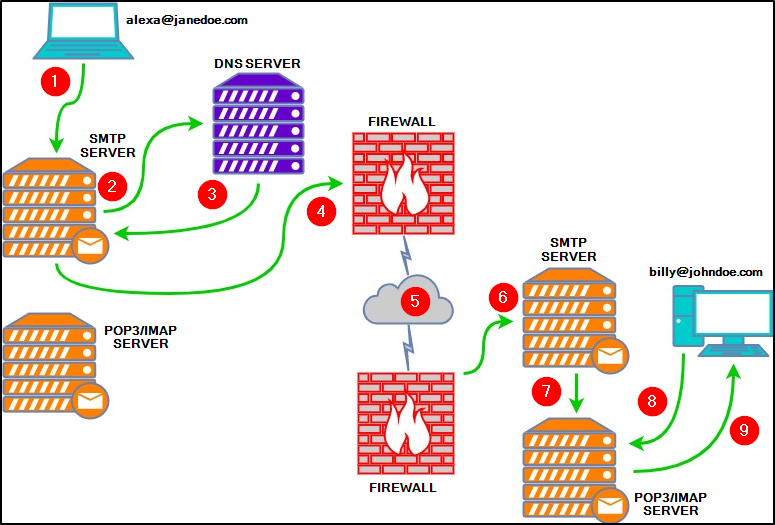
\includegraphics[width=\linewidth]{figs/email_flow.png}
    \caption{How email travels from the sender to the recipient.}
    \label{fig:c2:email_flow}
  \end{figure}

\subsection{Email structure}

Email communication is an integral component of modern digital communication, and now we know how this communication happens, understanding how an email travels from point A to point B and the protocols involved in the process. However, it is also important to understand the structure of an email and the information it contains. The standard format of email messages is known as \ac{imf}. As specified in \ac{rfc} 5322~\cite{rfc5322}, it defines the required headers and bodies for messages, as well as the content and syntax for different headers. There is also the \ac{mime} standard, which extends the capabilities of email to include multimedia content and non-ASCII text. It allows for the formatting of multipart messages and the inclusion of various types of binary files like images and documents. 
%\ac{mime} is defined in \ac{rfc} 2045~\cite{rfc2045}, \ac{rfc} 2046~\cite{rfc2046}, \ac{rfc} 2047~\cite{rfc2047}, \ac{rfc} 4288~\cite{rfc4288}, and \ac{rfc} 4289~\cite{rfc4289}.

Such protocols and formats led to the development of various email storage and exchange formats, notably \ac{eml} and \ac{mbox}. These formats utilize the foundational principles of these protocols to manage and store email data effectively.

% informação do livro https://www.dpconline.org/docs/technology-watch-reports/739-dpctw11-01-pdf/file
The \ac{eml} format typically stores each email message as an individual file, incorporating the standardized headers and body prescribed by the \ac{imf}. Attachments in \ac{eml} files are either included as \ac{mime} content within the message or referenced as separate files. \ac{mbox} combines all the emails in a folder into a single file. Although \ac{eml} and \ac{mbox} have gained widespread acceptance as standard formats because of their interoperability with current email clients, their approaches to email storage are different. Considering that \ac{mbox} is a method that keeps several emails in a file, handling each one separately may provide issues, while the individual file storage in \ac{eml} offers more granularity.
Also, it is appropriate to address the \ac{pst} format, which is primarily utilized by Microsoft Outlook. \ac{pst} files contain not just emails but also contacts, tasks, notes, and calendar events all in one file.

The selection of email format is crucial for efficient data administration and analysis when creating a system for phishing email detection. The decision to choose the \ac{eml} format over \ac{mbox} is motivated by the particular advantages it provides, especially about the granularity, providing large information about an email. The standardized nature of \ac{eml} files ensures broad compatibility with a variety of email clients beyond Microsoft Outlook, which is not the case with the \ac{pst} format. For a phishing email detection system that would need to process data from several sources, this compatibility is essential.

%estrutura de um email
\ac{eml} files include all of the raw data that makes up an email, including the body content, headers, attachments and signatures. 

\begin{figure}[H]
    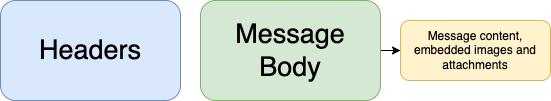
\includegraphics[width=\linewidth]{figs/eml_contents.png}
    \caption{Contents in \ac{eml} file.}
    \label{fig:c2:eml_contents}
  \end{figure}

The email headers contain details about the email servers that carried the email, thus serving as a digital trail of the email's journey from sender to recipient. This header is not just a single entity but a collection of various fields, each holding specific information.  Header fields are lines beginning with a field name, followed by a colon (":"), and followed by a field body, as specified in \ac{rfc} 5322~\cite{rfc5322}. The field name identifies the type of information, and the field body, following the colon, contains the specific details corresponding to the field name.
An example of an email headers message as an \ac{eml} file can be found in Figure \ref{fig:c2:eml}. Several fields are present in the email headers, each with its own purpose:

\begin{enumerate}[label=\Alph*]
    \item \textbf{Delivered-To}: The intended recipient's email address is contained in this email header field;
    \item \textbf{Received By}: This field contains the details of the last visited \ac{smtp} server, where the information revealed is the Server's IP address, \ac{smtp} ID of the visited server, and data and time at which the email was received by the \ac{smtp} server;
    \item \textbf{X-Received}: This field shares the IP address of the message-receiving servers, the \ac{smtp} ID of the server, and the date and time at which the email was received;
    \item \textbf{Return Path}: The return path is an email header that tells \ac{smtp} servers where they should send non-delivery notifications. According to RFC 5321,~\cite{rfc5321}, the return path consists of the sender’s mailbox;
    \item \textbf{Received From}: It has some information about the IP address of the sender along with other details like the hostname. Every server that handles this mail adds this header;
    \item \textbf{Received-SPF}: The system forwards the message only after the sender's identity is authenticated with the \ac{spf}. \ac{spf} is designed to verify that the sending server is authorized to send emails on behalf of the domain in the "From" address. It uses the domain address for authentication and adds the check status in the header field; 
    \item \textbf{Authentication Results}: \ac{mtas} apply a slew of authentication techniques to the email messages before processing them and add the results to this header field. It shares the ID of the authentication-performing server, the authentication techniques along their results;
    \item \textbf{From}: This field contains the sender's email address, indicating who sent the email;
    \item \textbf{To}: This field contains the recipient's email address;
    \item \textbf{Subject}: The subject line of the email offers a summary or a title to the email's content;
    \item \textbf{Date}: This indicates when the email was sent, providing a timestamp for the communication;
    \item \textbf{Message-ID}: It is the email's distinct ID that allows for differentiation. The same message ID cannot be shared by two emails;
    \item \textbf{MIME-Version}: This demonstrates that the message is prepared with the Multipurpose Internet Mail Extension (MIME) and supports a variety of forms, including audio, video, and plain text files.
\end{enumerate}

Depending on the email delivery service, custom headers can be included and are called X-Headers. The primary purpose of X-headers is to address the specific requirements of the sender that are not covered by the standard headers.

%eml file example

\begin{figure}[H]
  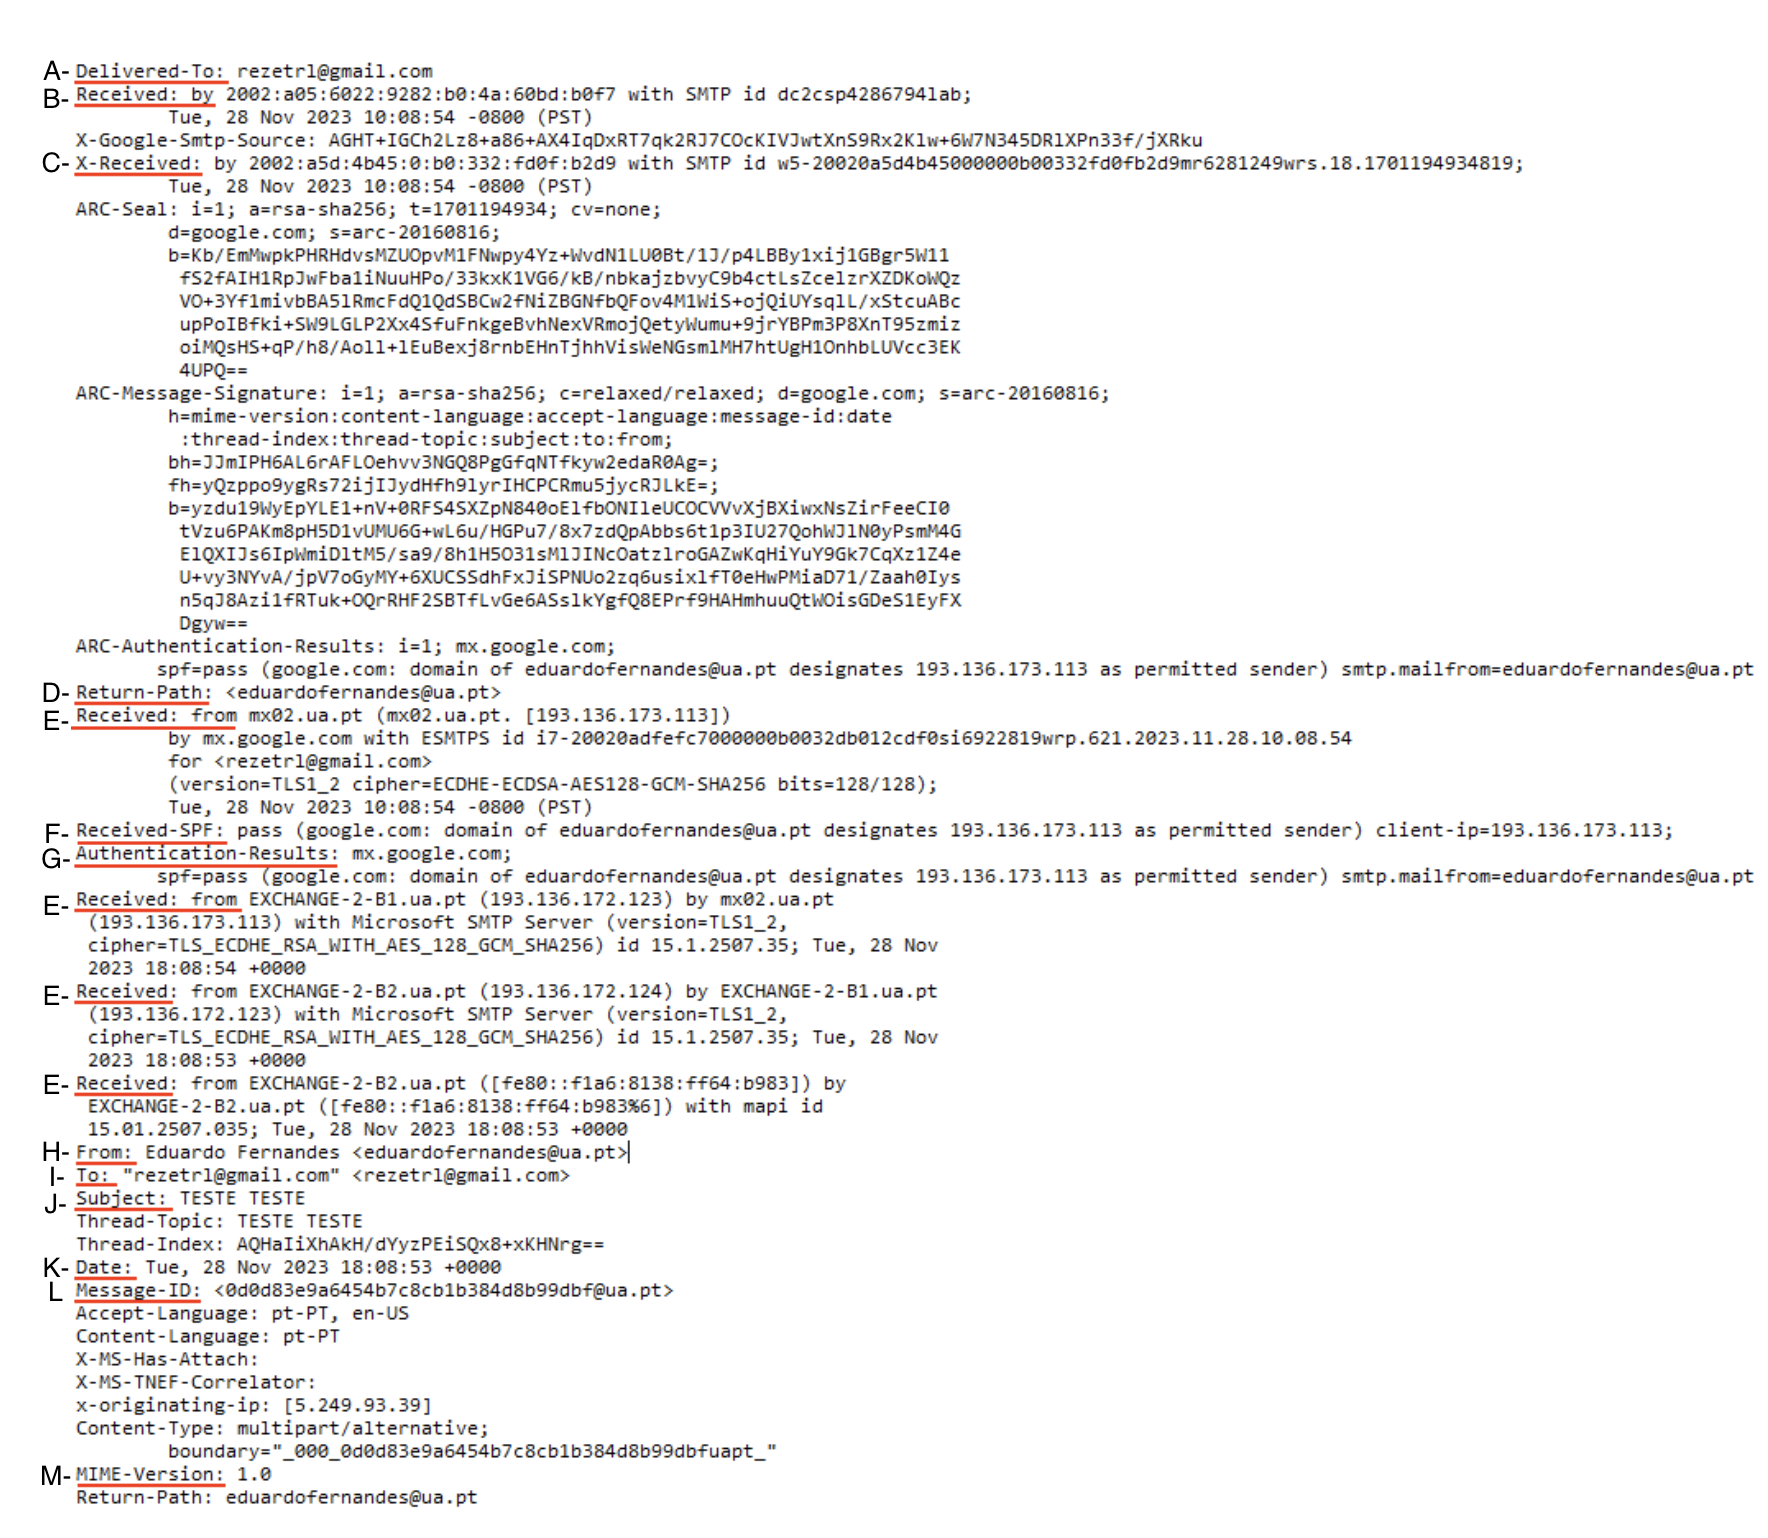
\includegraphics[width=\linewidth]{figs/eml.png}
  \caption[EML file example]{Email headers as an \ac{eml} file example.}
  \label{fig:c2:eml}
\end{figure}

As was discussed previously, the email content offers a wide range of information that can be crucial for detecting phishing emails. Besides the headers, the email body also contains equally pivotal information for detecting phishing attempts. While the email headers provide critical metadata, the body of an email often contains the substantive content that is essential for a more comprehensive analysis.

Contents of the email body are described by its \textbf{Content-Type} field, which indicates the respective formats of the information. The structure of the \textbf{Content-Type} consists of a \textbf{type} and a \textbf{subtype}, two strings, separated by a ‘/’, where no space is allowed between them. The type represents the category and can be a discrete or a multipart type, and the subtype is specific to each type. Discrete types are types that represent a single file, such as a single text or music file, or a single video. A document that is divided into several separate sections, each of which could have its own unique MIME type, is represented by a multipart type.

The list of discrete types is long but some important content-types are mentioned below:

\begin{itemize}
    \item \textbf{text}: Represents format which is human-readable. Includes subtypes such as "text/plain", "text/html", "text/css", and "text/javascript";
    \item \textbf{image}: Represents image of any type. Common subtypes examples are "image/jpeg", "image/png", and "image/svg+xml";
    \item \textbf{audio}: 	Represents any audio file format. Subtypes examples include "audio/mpeg", and "audio/wav";
    \item \textbf{application}: Represents any kind of binary data. Generic binary data is represented with the "application/octet-stream" subtype. Other common examples include "application/pdf", and "application/zip".
\end{itemize}

\begin{figure}[H]
    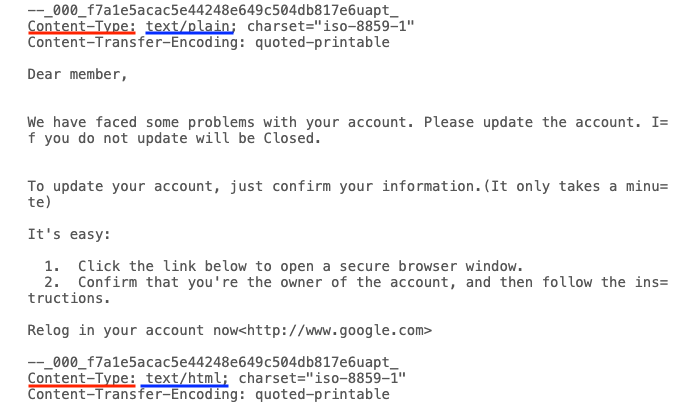
\includegraphics[width=\linewidth]{figs/eml_body.png}
    \caption{Email body in an \ac{eml} file example.}
    \label{fig:c2:eml_body}
  \end{figure}

Expanding the in-depth analysis of the email body, it is equally important to delve into the structure and representation of attachments in \ac{eml} files. The attachments contained in the email file are encapsulated within the message body, marked by their Content-Type (\textbf{A}) and Content-Disposition (\textbf{B}). The \textbf{A} header specifies the media type of the file, which is crucial in understanding the nature of the attachment. The following example in Figure \ref{fig:c2:attachement} indicates that the attachment is a PDF file, with a given name ("matter.pdf"). Also, the \textbf{B} header plays a critical role in how the attachment is processed by the email client, suggesting that the file should be treated as an attachment and not as an inline element. The 'filename' parameter provides the suggested name for the file when saved. Finally, the Content-Transfer-Encoding (\textbf{C}) header indicates that the file is encoded in base64, which is a common encoding technique that ensures the binary data of the attachment is transmitted over the network in a text format.

\begin{figure}[H]
    \begin{center}
        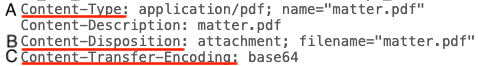
\includegraphics[width=12cm]{figs/attachment.png}
        \caption{Attachment example in \ac{eml} file.}
        \label{fig:c2:attachement}
    \end{center}
  \end{figure}

\begin{comment}
The EML (Email) is a common format for all types of email software. We can think of the
EML file as a file generated after the email is archived, retaining the original HTML format and title, and so forth. The basis of our detection system is the EML file, which provides us with large email-related information. Fortunately, most mail systems provide a window to download EML files directly. Besides, when the user logs in to the mailbox client, the EML file is automatically downloaded to the local.
Each EML file has a standard format, which allows it to load by specified rules. In the EML file, some of the information is base64 encrypted, so it needs to be decrypted to get the rawest data. In the process of extracting, the email file that missing field values will be considered abnormal data and be discarded.
\end{comment}

\subsection{Email features for phishing detection}

% perceber o que faz com que as pessoas caiam em phishing (tecnicas de phishing e que metadados podem ajudar nestas tecnicas)

Email metadata plays a critical role in the field of email phishing detection. All the fields explained before, including headers and other structural components, can offer information to determine the authenticity of an email. This metadata, which users frequently ignore, includes details such as the sender's address, routing information, timestamps, and more, giving information to help comprehend an email's origin and path.

Email spoofing is a very common type of phishing technique. It is a threat that involves sending email messages with fake information on email headers. Because a spoofed email and regular mail are similar in many aspects, email spoofing takes advantage of these similarities. Attackers can customize the information in several fields such as "Return-Path", "Reply-To", "From", "Subject", "Date", and "To".
The "Return Path" is where bounce messages go if the email fails to deliver. In legitimate emails, the "From" and "Return-Path" are typically consistent, representing the same source. However, in the case of email spoofing, there is often a discrepancy between these two fields. Scammers frequently manipulate the "From" address to appear as a trustworthy source, although they forget to modify the "Return-Path".
One of the main warning signs is an inconsistency between the "Reply-To" and "From" addresses. This disparity suggests the sender might be attempting to hide their true identity, which is a common phishing attempt approach. Additionally, if the “From” address does not align with the entity the email claims to represent, it further raises even more questions about the email's credibility. 
Another important detail is the nature of the "Subject" line. Phishing emails frequently have subject lines that are concerning, urgent, or too appealing in an attempt to get the receiver to act immediately without closely examining the legitimacy of the email. 
The "Date" field also needs to be taken into consideration. Attackers might use data that are not logical, including dates in the future or the past. Also, if the “To” address does not specifically name you, it can be indicative of phishing. Phishing emails often lack specific identification of the recipient, suggesting a broad targeting strategy known as mass mailings.

Another technical aspect of the email's metadata that can provide important information is the \ac{spf}. A "Fail" or "SoftFail" status from the \ac{spf} check, or a lack of \ac{spf} validation, raises serious questions about the legitimacy of the email. Also, another important point is that the IP address must line up with the sender's email service. If this does not happen, it suggests that the email may have been sent from an unauthorized or suspicious server. The "Received" fields can also provide crucial information, tracing the email's path across the internet. Unknown servers along this path, especially at the beginning or end, suggest that the email routing process may be compromised, raising the possibility of a phishing attempt.\\

% falar sobre features utilizadas em outros trabalhos

\citet{8257764} categorized the spam features into three primary groups based on the examination of the features present in the relevant studies in their literature: attachment features, payload (body) features, and header features. The header features were grouped into two classes, called email metadata and subject, and are displayed in Figure~\ref{fig:c2:header_features}.

\begin{figure}[H]
    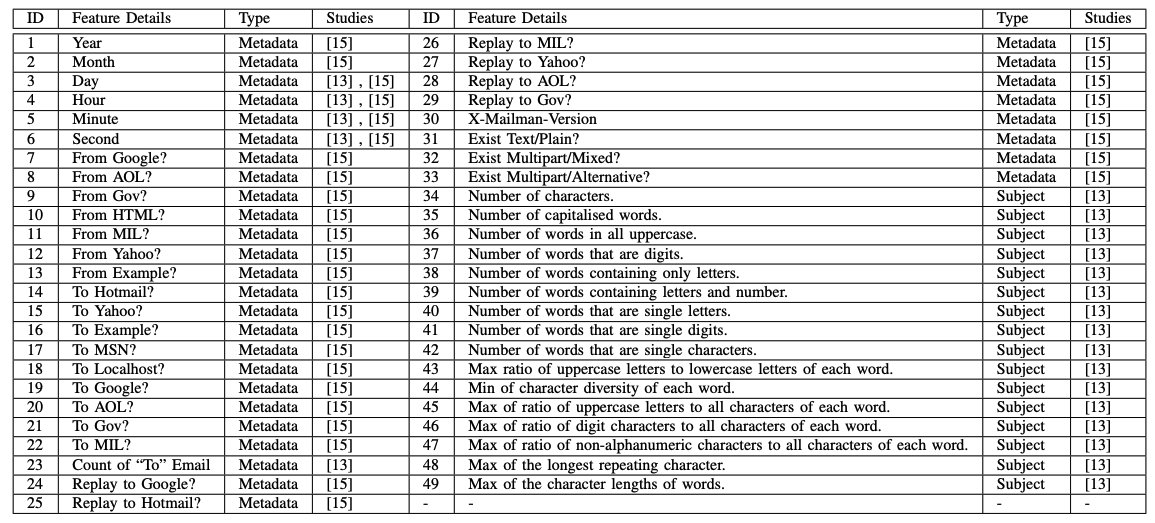
\includegraphics[width=\linewidth]{figs/headers_article.png}
    \caption{\citet{8257764} proposed header features.}
    \label{fig:c2:header_features}
  \end{figure}

\citet{Abadla202312} in their study, used a dataset that has around 3800 records and 31 features related to the body of the email message, the subject box, and the sender’s address.
The proposal highlights specific characteristics often found in phishing emails, such as the inclusion of words like "urgent" and "suspension" in the subject line. Attackers deliberately use these terms to make victims frightened and force them to act right away. In addition, they identified that phishers use header phrases like "Fwd: mail" and "Re: mail" to create the sense of a continuing conversation, which increases the possibility that the receiver may interact with the email. This analysis of header features is crucial in understanding the linguistic and psychological strategies used in phishing attacks, thereby aiding in the development of more effective detection mechanisms. They introduced also the concept of “subject richness”, which pertains to the ratio of the number of words to the number of characters in the subject line. Turns out that this feature is crucial as it influences the open rate of an email.

In the context of phishing detection, the "Content-Type" field within attachments is a significant indicator. 
Phishing emails may contain attachments with content-types that are commonly associated with executable or scriptable content, such as "application/x-msdownload" for executables or "application/x-shockwave-flash" for Flash objects, which are potentially harmful. Moreover, attackers may disguise malicious attachments with a benign-looking content-type, such as "application/pdf" or "image/jpeg", while the actual file is a harmful executable. As mentioned in~\citet{caldwell2013spear} work, the attachment serves as the ideal camouflage for introducing an advanced persistent threat, commonly disguising itself as either a PDF file or a potentially flawed Office document, appearing subtle enough for people to accidentally execute. 

In the~\citet{dewan2014analyzing} study, a significant portion is devoted to analyzing the attachment names and types in spear phishing emails. The study highlights a clear distinction between the attachment names used in spear phishing and general spam or phishing emails. Spear phishing emails tend to have attachment names that appear more realistic and genuine, as opposed to the more irrelevant and lengthy names found in general spam or phishing emails. This difference in naming conventions indicates that spear phishing attacks are crafted with more effort to make them appear legitimate and trustworthy, thereby increasing the likelihood of the recipient opening the attachment. Additionally, the paper discusses the types of file formats commonly used in these emails. Both spear phishing and general spam/phishing emails prominently feature executable (.exe, .bat, .com) and compressed (.rar, .zip, .7z) file types, along with common document formats like Microsoft Word, Excel, PowerPoint, and PDF files. The research explores the presence of attachments in the email body, indicating whether an email contains an attachment, and this feature, among others, is used to analyze and classify emails in their dataset. Although they do not use the attachment name and type as features for their classification, they can be used to enhance the detection of phishing emails.

The proposal presented by~\citet{li2020lstm} delves into the complexities of detecting phishing emails, particularly focusing on the role of email attachments in these malicious activities. In addressing this challenge, they propose an email feature extraction algorithm that focuses on various aspects of emails, including the names and suffixes of attachments. In the end, they got high accuracy results, which demonstrates the effectiveness of their approach, especially in the context of detecting phishing emails with attachments.

\begin{comment}
Therefore, it is crucial to not only inspect the declared \textbf{Content-Type} but also to perform a deeper analysis of the attachment itself. 
This can include scanning for known malware signatures, analyzing the file's actual content beyond its MIME declaration, and sandbox testing to observe the file's behavior when opened. By combining these techniques, a more robust and accurate detection of phishing attempts can be achieved, enhancing the security of email communication.
\end{comment}

\begin{comment}
The first step is to understand why people fall for phishing. Something in phishing emails lures the victims into clicking on some malicious link or providing confidential information.~\citet{butavicius2022people} performed a study where the objective was to understand why that happens. For that, they conducted an online experiment, and participants underwent an email classification task designed to examine susceptibility to phishing. In the study's discussion, it was mentioned that participants phishing email detection skills were poor. They correctly identified phishing only 42\% of the time and incorrectly flagged emails that were legitimate 31\% of the time. Despite the emails having leakage cues such as poor grammar, spelling, and punctuation the majority still fell for the attack and clicked the fake malicious link provided. 
\end{comment}


% \section{Existing tools and platforms}
% ThePhish - GitHub

\section{AI for Phishing Detection}

% continual learning pode ser uma hipótese para o modelo ir aprendendo (continual learning vs reinforcement learning vs transfer learning)

As phishing techniques evolve and become increasingly sophisticated, traditional methods like rules-based filters and signature detection are no longer enough to keep us safe. This is where \ac{ml} and \ac{dl} come into play as powerful tools that can enhance our ability to detect phishing attacks. These artificial intelligence techniques enable systems to learn and adapt, allowing them to recognize subtle patterns and anomalies that may trick traditional detection approaches.
By incorporating \ac{ml} and \ac{dl} into phishing detection, we not only aim to address the difficulties of identifying these deceitful communications but also play a crucial role in strengthening cybersecurity measures.

\subsection{Natural Language Processing}

% falar de coisas gerais sem entrar muito em detalhe

% descrição do que é nlp
As a branch of artificial intelligence, \ac{nlp} focuses on the interaction between computers and human language.

\ac{nlp} combines the power of linguistics and computer science to enable machines to understand, interpret, and respond to human language in a valuable and meaningful way. Human signs and languages, such as voice, writing, and text, can be automated with a certain level of accuracy using \ac{nlp} techniques~\cite{Sathish20231612}.

% o que é que o nlp pode fazer para detetar phishing
The relevance of \ac{nlp} in detecting phishing emails is based on its ability to analyze and understand the textual content of emails. Phishing emails frequently include linguistic clues different from those in normal correspondence, and trick recipients into revealing sensitive information. These cues can be subtle, such as the use of specific words or phrases, or more obvious, such as poor grammar and spelling. In either case, these linguistic features can be used to identify phishing emails and \ac{nlp} techniques can be used to extract and analyze them.

% falar do processo de nlp e de algumas técnicas utilizadas
The \ac{nlp} field is vast and has a wide array of techniques, each contributing uniquely to the understanding and processing of language in the \ac{nlp} process. Data preprocessing is one step in \ac{nlp} that involves cleaning and transforming raw data into a format that can be understood and used by models. Some of the techniques used in this step include tokenization, normalization, stemming, the use of stop words, the application of regular expressions and both syntactic and semantic analysis.
Feature extraction is another important step in \ac{nlp} that involves the extraction of features from the text. These features can be used to train \ac{ml} models to perform various tasks in this field. Techniques such as bag-of-words, word embeddings, and TF-IDF are used to extract features from text.
After this, numerical features extracted by the previous techniques can be fed into \ac{ml} models. Depending on the task, different models can be used, such as classification, clustering, and regression models.

% mostrar aplicações de nlp com machine learning
\citet{Vazhayil201869} presents an insightful application of \ac{nlp} methods in conjunction with \ac{ml} models for phishing email detection. This study uses Term Document Matrix (TDM) for the non-sequential representation of the corpus, followed by Singular Value Decomposition (SVD) and Nonnegative Matrix Factorization (NMF) to extract important features. These extracted features were then used to train various \ac{ml} algorithms, including \ac{dt}, \ac{knn}, \ac{nb}, \ac{rf}, \ac{svm}, and \ac{lr}. In the conclusion, they highlighted the effectiveness of this approach in distinguishing phishing emails from legitimate ones. However, the paper also acknowledges a limitation: the reliance on feature selection, which requires domain knowledge. To address this, future work could incorporate \ac{dl} models that can learn more complex patterns directly from the raw data, potentially improving efficacy. \citet{Gutierrez2018988} mentioned that the most common defensive approaches frequently display a lack of adaptability. This is primarily because of its basis in rigid frameworks like regular expressions that recognize specific text patterns. A major flaw with \ac{nlp} developed on \ac{ml} is their reliance on surface-level text analysis rather than exploring deeper semantics. This means that if different synonyms of words are chosen or the sentence construction is changed, it is difficult for \ac{nlp} built on \ac{ml} to analyze these changes.

% mostrar aplicações de nlp com deep learning
Advancements in this area have led to the development of more sophisticated techniques. Unlike traditional \ac{ml} models, \ac{dl} models can automatically detect and learn features from raw text, allowing them to capture complex relationships between words and phrases in a language and to generalize to new and unseen examples. Some examples of \ac{dl} models that can be used in \ac{nlp} are \ac{rnn}, \ac{cnn} and transformer models. \ac{rnn} is a type of neural network that can process sequential data, such as text, by using a hidden state to store information about previous inputs. \ac{cnn}, typically known for image processing, have also been effectively repurposed for \ac{nlp} tasks. Moreover, the emergence of Transformer models marks a significant leap. These models excel in understanding the context of language, processing each word concerning all other words in a sentence, and using self-attention mechanisms to capture the global relationships in a sentence.

% ver melhor este texto
\begin{comment}
    \citet{Gutierrez2018988} mentioned that the most common defensive approaches frequently display a lack of adaptability. This is primarily because of its basis in rigid frameworks like regular expressions that recognize specific text patterns. This limitation highlights how important it is to find different methods to improve phishing detection. The problem with already existing automated solutions, built to manage the flood of phishing emails, is to quickly detect unseen phishing attempts. A major flaw in these solutions is their reliance on surface-level text analysis rather than exploring deeper linguistic patterns and deceitful strategies, such as the use of synonyms and varied sentence structures.
    In the proposed solution they used advanced \ac{nlp} techniques like Named Entity Recognition that its used to recognize different entity types, such as persons, locations, organizations, within the text, and Freebase that essentialy returns potential categories the entity belongs to and provides a score of how relevant each category is. These two techniques form a set of higher-level features, that also includes synonym substitution, to better understand the semantics of phishing emails.
\end{comment}


\subsection{Machine Learning approaches}


The work proposed by~\citet{rabbi2023phishy} aims to find the most efficient techniques for preventing phishing attacks. For that, six \ac{ml} algorithms were separated including \ac{lr}, \ac{knn}, \ac{ab}, \ac{mnb}, \ac{gb}, and \ac{rf}. One of the goals was to answer what is the most powerful \ac{ml} algorithm for detecting phishing emails and the results showed that the \ac{rf} performed better than other \ac{ml} algorithms having 98.38\% accuracy and a low rate of false negatives. Although \ac{rf} obtained better results, its training time is relatively long when compared to others. However, the approach solely focuses on the email body features. There is more information such as the sender details, header information, and URLs in the email that can provide useful information for the model and increase performance.

In their study, the authors of~\cite{Kumar2023222} introduced a phishing URL detection method that integrates multiple \ac{ml} algorithms with unique hybrid features. These hybrid features are generated by first applying \ac{pca} to word vector features, and then merging them with \ac{nlp} features. The dataset used in this study comprises approximately 37,000 URLs, evenly split between phishing and legitimate sites. Word vectors, also known as word embeddings, numerically represent words in a high-dimensional space. \ac{pca} is employed to reduce the dimensionality of these vectors. The resultant hybrid feature set, post-merging with \ac{nlp} features, encompasses 142 distinct features. Among the various \ac{ml} algorithms evaluated, the \ac{rf} algorithm exhibited the highest accuracy, achieving a remarkable 99.75\%.

\citet{Shaukat2023} proposed a solution that uses a three-layered approach to detect phishing websites. This multi-perspective layered evaluation has three layers: URL layer, text layer, and image layer. The first one analyzes URL features to detect phishing URLs, the second layer looks for spam content in website text by using \ac{nlp} and the last one categorizes the content of websites by processing text and graphics from advertising. The PhishTank dataset containing 20,000 phishing URLs and the SMS spam and ham dataset from Kaggle were used to train the machine learning models for the first two layers. The third layer takes the images from the websites as input to convert them into text so that they can be readable and given as input to the second layer model. For the URL classification the \ac{dt}, \ac{rf}, \ac{mp}, \ac{svm}, \ac{lr} and XG Boost models were tested. \ac{nb} and Linear \ac{svc} models were used in the second layer to perform phishing text classification. The results showed up to 91.2\% accuracy in the detection of legitimate or phishing URLs with XGBoost, and 98.9\% accuracy with the Linear \ac{svc} model in the text analysis step.

\citet{Karhani2023206} presents a novel approach to detecting phishing URLs and SMS-based phishing (smishing) attacks. This approach combines domain-related features with \ac{nlp} techniques. The features related to domains are extracted and used alongside \ac{nlp}, which is trained on actual smishing messages, to detect attacks accurately. The study proposes integrating this detection system with the open-source \ac{misp}. This integration enhances the storage and utilization of flagged phishing domains.
The dataset for this study includes data from TELUS Corporation and publicly available sources, featuring a mix of phishing and legitimate domains and SMS messages. The methodology involves a hybrid model that combines a \ac{dt} model and an \ac{nlp} model using \ac{svc}.
The model demonstrates an impressive accuracy of 99.40\% and an F1 score exceeding 99\%. The domain checker, part of the hybrid model, showed notable generalization capabilities with an F1 score of 99.01\% and an accuracy of 98.04\%.
The \ac{nlp} checker, while effective, did not generalize as well to the confirmed phishing dataset provided by TELUS, with an F1 score and accuracy of 92.98\% and 86.88\% respectively.
When both models were combined, the \ac{nlp} checker effectively corrected 69.35\% of the domain checker's false negatives, improving the final accuracy to 99.40\%.
%The importance of this work lies in its high accuracy and practical application in real-time phishing detection. The integration with MISP and the combination of domain and NLP features represent an effective approach to tackling phishing threats.

\subsection{Deep Learning approaches}

The authors of~\cite{Benavides-Astudillo2023} developed a phishing detection model focusing on the text of web pages rather than URL addresses. This model uses \ac{nlp} and \ac{dl} algorithms, specifically using the Keras Embedding Layer with \ac{glove} to exploit semantic and syntactic features of webpage content. The method involves four phases: word parsing, data pre-processing, feature representation, and feature extraction. This approach ensures that important words and the order in which they appear are both considered for analysis.
The model's performance was evaluated using four DL algorithms: \ac{lstm}, \ac{bilstm}, \ac{gru}, and \ac{bigru}. Notably, all four algorithms achieved a mean accuracy of at least 96.7\%, with \ac{bigru} emerging as the top performer, achieving an accuracy of 97.39\%.
Further analysis revealed that both \ac{gru} and \ac{bigru} consistently outperformed \ac{lstm} and \ac{bilstm} in terms of test accuracy. Notably, \ac{gru} demonstrated the fastest training time, completing its training in just 240 seconds, which could be beneficial if rapid processing is required.

\citet{ALHOGAIL2021102414} detailed an approach using \ac{dl} algorithms and \ac{nlp} to enhance phishing detection. \ac{dl} techniques are useful for phishing email detection because they perform especially well with unstructured data, like email content. The study highlights the advantages of \ac{dl} over other machine learning algorithms because traditional approaches require significant feature engineering. The core of this approach involves a \ac{gcn}, which is described as a type of \ac{cnn} that operates directly on graphs. By utilizing a single large graph made from the entire email corpus, it converts the document classification problem into a node classification problem. This study uses \ac{nlp} on email body features alongside \ac{dl} algorithms using \ac{gcn} to build an effective phishing email detection classifier. The proposed classifier is built through three main phases: data collection and preparation, construction of the detection model using \ac{dl} \ac{gcn} algorithms and testing the classifier in a supervised approach using testing data for validation. This model demonstrates its effectiveness in detecting phishing emails based solely on body text, achieving an impressive accuracy rate of 98.2\% with a low false-positive rate of 0.015.

The work presented by~\citet{8701426} introduces THEMIS, a new phishing email detection model, which utilizes an improved \ac{rcnn} combined with a multilevel vector approach and an attention mechanism. The model analyzes the email structure, focusing on four detailed parts: the email header, the email body, and text at both the word and character levels.
The THEMIS model, combining multilevel embedding with the improved \ac{rcnn}-Attention model, vectorizes the email's text structure and applies \ac{bilstm} for better email representation. The attention mechanism is applied between the email header and body, allowing the model to prioritize more significant information from these parts. This complex approach enables THEMIS to perform exceptionally well on an unbalanced dataset, achieving an accuracy rate of 99.848\% and a very low false positive rate (FPR) of 0.043\%, which shows its effectiveness in accurately identifying phishing emails while minimizing the misclassification of legitimate emails.

\citet{atawneh2023phishing} proposal explores the use of \ac{dl} techniques, including \ac{cnn}, \ac{lstm} networks, \ac{rnn}, and \ac{bert}, for detecting email phishing attacks. The proposed model in the study involved collecting, preparing, and utilizing a dataset for training and testing the previously mentioned \ac{dl} models for phishing detection. This included steps like dataset acquisition, data preparation, feature extraction, and model training and testing. The research involved removing HTML tags, numbers, punctuations, stop words, and infrequent words from the email datasets. Stemming was also applied to reduce words to their base form. These preprocessing steps were essential for reducing noise in the data and enabling effective learning by the \ac{dl} models. All these models achieved high accuracy, with the best performance observed using \ac{bert} and \ac{lstm}, reaching an accuracy of 99.61\%.

Table~\ref{tbl:c2:comparison_table} summarizes the proposed works discussed in this section related to phishing detection. The literature review revealed several machine learning and deep learning techniques that can be used to detect phishing emails. It also evaluated the performance of various techniques in terms of accuracy.

% alterar a tabela para os papers certos
\begin{table}[ht]
    \centering
    \caption{Summary of the discussed works.}
    \label{tbl:c2:comparison_table}
    \begin{tabular}{p{4cm}p{4cm}p{4cm}p{2cm}}
    \hline
    \textbf{Authors} & \textbf{Purpose} & \textbf{Major Theme} & \textbf{Accuracy} \\
    \hline
    Zamir et al., 2020 [6] & Phishing website detection & Using machine learning and neural networks & 97.40\% \\
    \hline
    Valecha et al., 2021 [14] & Phishing email detection & Machine learning models & 96.52\% \\
    \hline
    Barushka \& Hajek 2018 [15] & Categorizing spam and non-spam messages & Integration of DBB-RDNN-ReL for feature selection & 98.51\% \\
    \hline
    Fang et al., 2019 [16] & Detecting phishing emails & Use of diversified datasets & 99\% \\
    \hline
    Alhogail \& Alsabih et al., 2021 [17] & Email phishing detection and deep learning & Natural language processing and graph conventional network & 98.2\% \\
    \hline
    \end{tabular}
    \end{table}

\section{Sentiment analysis}

% o que é sentiment analysis
Sentiment analysis is a \ac{nlp} technique that refers to the process of evaluating and determining the sentiment, which is characterized as feeling or emotion, contained in a certain text.
The core of sentiment analysis lies in polarity detection, which classifies text into basic categories like positive, negative, or neutral. However, sentiment analysis goes beyond polarity to identify particular emotions like happiness, frustration, anger, and sadness. This technique can be applied to a wide range of domains, including social media, customer reviews, and emails.

% como funciona sentiment analysis (ver aqui https://monkeylearn.com/sentiment-analysis/)
Generally, the input to a sentiment classification model is a piece of text, and the output is the probability of a certain sentiment or emotion. Typically, this probability is based on either hand-generated features, word n-grams, TF-IDF features, or using \ac{dl} models to capture sequential long- and short-term dependencies. Many emotion systems use lexicons, which are lists of words and their corresponding emotions. These lexicons can be used to determine the sentiment of a text by counting the number of words that match the words in the lexicon. However, this approach is limited by the fact that it does not consider the context of the words, which can lead to inaccurate results.

% desafios de sentiment analysis
Despite its wide applications, sentiment analysis faces several challenges. One of the most significant is detecting sarcasm and irony, as these often convey the opposite meaning of the literal words used, leading to potential misinterpretation. Additionally, sentiment analysis must contend with contextual and cultural variations. The same phrase may carry different meanings in different cultures or situations, complicating universal model applicability. Moreover, because human language can be unclear and different people might see it differently, sentiment analysis becomes more complicated. What is considered a positive sentiment in one context may be neutral or even negative in another, which is why we need advanced models that understand the context.

% téncicas de sentiment analysis


% exemplos de artigos que fazem sentiment analysis
% ver melhor esta parte
The~\citet{SAILUNAZ2019101003} study provides a robust example of an integrated approach. The researchers focused on extracting sentiment and emotion from tweets and replies on specific topics. This involved creating a dataset encompassing text, user emotion, sentiment information, and various other parameters.

A specific example is the Sentiment Analysis Module detailed in the~\citet{10085351} study, where this module captures the emotions or sentiments expressed in emails. It employs the \ac{nltk}, an open-source Python library, to analyze the text based on common and repetitive sentiment words included in the training set. Determining sentence polarity is an important part of this module since it helps to comprehend the emotional tone that an email provides. The system pre-determines the polarity of specific polar words to interpret the sentiment accurately. 



\section{Insights}

One important finding from the state-of-the-art (SOTA) analysis is that there are no tools that can both detect phishing emails and perform sentiment analysis at the same time. Sentiment analysis, as defined previously, involves the process of discerning the underlying sentiment or emotion embedded in textual content, such as emails. This process is not merely about polarity detection (classifying text as positive, negative, or neutral) but extends to identifying specific emotions like happiness, frustration, anger, and sadness. Existing phishing detection systems do not perform this type of analysis, which is crucial in understanding the psychological strategies used in the attacks. This is a significant gap in the literature that we aim to address in this study.

The need for a model that continuously adjusts to the constantly evolving field of phishing tactics is equally essential. This adaptive approach is not just a technological improvement but a strategic necessity in the ongoing battle against these cyber threats.

%The continual learning approach is a promising solution to this challenge, as it enables the model to learn from new data and adapt to new situations. 